\chapter{Kravspecifikation}

I projektet er det valgt at benytte user stories til at beskrive den ønskede funktionalitet. Disse stories er lavet på baggrund af MoSCoW analysen. Ikke alle userstories er taget med i denne analyse da eksempelificeringen igennem hele rapporten af enkelte user stories, ville være mere beskrivende. På figur. \ref{fig:KontekstDia} ses systemets aktør kontekst diagram. For en fuld liste af User stroies henvises til dokumentationen

\begin{figure}[H]
	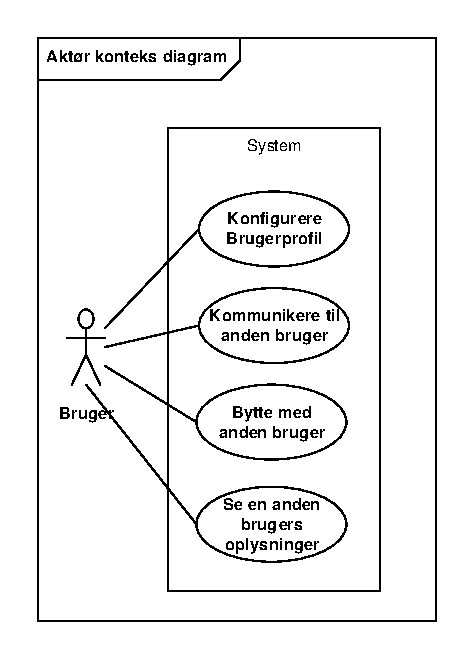
\includegraphics[trim = 6mm 6mm 6mm 6mm, clip, width=100mm]{../Dokumentation/figures/KontekstDiagram.PDF}
	\caption{Aktør kontekst diagram}
	\label{fig:KontekstDia}
\end{figure}

\section{Oprette en bytteannonce}
{\color{blue}\textbf{EGENSKAB}:} Oprette en bytteannonce \\
Som bruger \\
Ønsker jeg at kunne oprette en bytteannonce \\
For at kunne bytte med andre brugere af systemet.\\ \\
{\color{blue}\textbf{BAGGRUND}} \\
{\color{blue}\textbf{Givet}} at bruger er logget ind \\ \\
{\color{blue}\textbf{SCENARIE:}} Oprette en bytteannonce \\
{\color{blue}\textbf{Når}}  bruger ønsker at oprette en bytteannonce i systemet \\
{\color{blue}\textbf{Så}} navigerer han til menupunktet ”Opret annonce” \\
{\color{blue}\textbf{Så}} udfylder han bytteannonce-skabelonen \\
{\color{blue}\textbf{Og}} trykker på ”Opret annonce”-knappen
\section{Søg efter bytteannoncer}
{\color{blue}\textbf{EGENSKAB}:}Søg efter bytteannoncer \\
Som bruger \\
Ønsker jeg at kunne søge efter bytteannoncer \\
For at kunne finde en bestemt type vare\\ \\
{\color{blue}\textbf{BAGGRUND}} \\
{\color{blue}\textbf{Givet}} at bruger er logget ind \\
\\
{\color{blue}\textbf{SCENARIE:}} Søg efter bytteannoncer \\
{\color{blue}\textbf{Når}} bruger ønsker at søge efter bytteannoncer i systemet\\
{\color{blue}\textbf{Så}} navigerer brugeren til menupunktet ”Søg” \\
{\color{blue}\textbf{Så}} indtaster brugeren søgekriterier som består af(Kategori, afstand, evt byttegenstand)\\
{\color{blue}\textbf{Og}} trykker på “søg“-knappen

\section{Ikke-Funktionelle krav}
BargainBarter indeholder nogle ikke funktionelle, hvor alle her er opskevet.
\input{../Documentation/secions/ikke-funktionelle_krav.tex}